\section{Dynamical Variational AutoEncoders - Theory}\label{DVAEs}

\begin{frame}{Dynamical Variational Auto Encoders : generalities}
    \begin{itemize}
        \item <1-> Time : regular $t_1, t_2,... t_T$ or irregular $t_{i_1}, t_{i_2},..., t_{i_T}$ sampling times
        \item <1-> Observations : a sequence of $T$ points \textbf{$x_{1:T}$} $= \{(x_t)_{t=1,...,T}\}$ (or \textbf{$x_{t_{i_1}:t_{i_T}}$} $= \{(x_{t_i})_{i=1,...,T}\}) \in \mathbb{R}^F$.
        \item <1-> Latent variables : an associated sequence of $T$ latent variables \textbf{$z_{1:T}$} $= \{(z_t)_{t=1,...,T}\} \in \mathbb{R}^L$ (resp. $z_{t_1},..,z_{t_T}$)
        \item <1-> Optionally, a sequence of -usually deterministic- $T$ inputs $u_{1:T} = \{(u_t)_{t=1,...,T}\} \in \mathbb{R}^U$ (resp. $u_{t_i}, i=1,...,T$)
        \item <2-> \textbf{Encoding temporal dependency in prior over $z_i$'s}
        \item <2-> Arbitrary likelihood (observation model)
        \item <2-> Approximate posterior usually same form as true posterior
        \item <2-> Use \textbf{D-Separation} in \glsreset{gpm}\gls{gpm} to simplify expressions
        \item <2-> Untractable true posterior $\implies$ training by maximizing a \glsreset{vlb}\gls{vlb}
    \end{itemize}
\end{frame}

\begin{frame}{General formulation of DVAE}
    \begin{block}{Generative model}
        \begin{align}
            p(x_{1:T}, z_{1:T} \vert u_{1:T}) &= \prod_{t=1}^T p(x_t, z_t \vert x_{1:t-1}, z_{1:t-1}, u_{1:T}) \\
            &= \prod_{t=1}^T p(x_t \vert x_{1:t-1}, z_{1:t}, u_{1:T}) p(z_t \vert x_{1:t-1}, z_{1:t-1}, u_{1:T}) \\
            &= \prod_{t=1}^T p(x_t \vert x_{1:t-1}, z_{1:t}, u_{1:t}) p(z_t \vert x_{1:t-1}, z_{1:t-1}, u_{1:t})
        \end{align}
    \end{block}
    \textbf{Only assumption : causal dependency $x_t, z_t$ on inputs $u_{1:t}$ $\implies$ $\vert u_{1:T} = \vert u_{1:t}$.}

    (NB : assume no input in the rest of the presentation)
\end{frame}

\begin{frame}{Posteriors}
    \begin{itemize}
        \item <1-> True posterior  $p(z_{1:T} \vert x_{1:T})$ usually untractable::
            \begin{align*}
                p(z_{1:T} \vert x_{1:T}) &= \prod_{t=1}^T p(z_t \vert z_{1:t-1}, x_{1:T})
            \end{align*}
        % It can be noted that the true posterior exhibits a dependence of $z_t$ on \textit{past} $z_{1:t-1}$, but a dependence on the \textit{whole} data sequence $x_{1:T}$ (think Kalman smoother).
        \item <2-> Inference model : approximate posterior by an parametric encoder $q_{\phi}(z_{1:T} \vert x_{1:T})$ ($\phi$ the set of parameters):
            \begin{align*}
                q_{\phi}(z_{1:T} \vert x_{1:T}) &= \prod_{t=1}^T q_\phi(z_t \vert z_{1:t-1}, x_{1:T})
            \end{align*}
        \item <3-> D-separation on \gls{gpm} to simplify $p_{\theta_x}(x_t \vert x_{1:t-1}, z_{1:t})$ and $q_\phi(z_t \vert z_{1:t-1}, x_{1:T})$
        \item <4-> Good practice : use the true posterior expression $p(z_{1:T} \vert x_{1:T})$ for $q_\phi(z_t \vert z_{1:t-1}, x_{1:T})$
    \end{itemize}
\end{frame}

\begin{frame}{Likelihood}
    \begin{itemize}
        \item <1-> Observation model and encoder:
        \begin{align}
            p_{\theta}(x_{1:T}, z_{1:T}) &= \prod_{t=1}^T p_{\theta_x}(x_t \vert x_{1:t-1}, z_{1:t}) p_{\theta_z}(z_t \vert z_{1:t-1}, x_{1:t-1}) \\
            \label{q_phi_dev}
            q_\phi(z_{1:T} \vert x_{1:T}) &= \prod_{t=1}^T q_\phi (z_t \vert z_{1:t-1}, x_{1:T})
        \end{align}
        \item <2-> Log likelihood
        \begin{align}
            \log{p(x_{1:T})} &= \log{\frac{p(x_{1:T}, z_{1:T})}{p(z_{1:T} \vert x_{1:T})}} \\
            &= \E{q_{\phi}(z_{1:T}\vert x_{1:T})} \log{\frac{p(x_{1:T}, z_{1:T})}{q_{\phi}(z_{1:T}\vert x_{1:T})} \frac{q_{\phi}(z_{1:T}\vert x_{1:T})}{p(z_{1:T} \vert x_{1:T})}} \\
            &= \E{q_{\phi}(z_{1:T}\vert x_{1:T})} \log{\frac{p(x_{1:T}, z_{1:T})}{q_{\phi}(z_{1:T}\vert x_{1:T})} + \KL{q_{\phi}(z_{1:T}\vert x_{1:T})}{p(z_{1:T} \vert x_{1:T})}} \\
            &\geq \E{q_{\phi}(z_{1:T}\vert x_{1:T})} \log{\frac{p(x_{1:T}, z_{1:T})}{q_{\phi}(z_{1:T}\vert x_{1:T})}} = \VLB
        \end{align}
    \end{itemize}
\end{frame}

\begin{frame}{Variational Lower Bound}
    \begin{itemize}
        \item Lower bound:
        \begin{align}
            \VLB &= \E{q_{\phi}(z_{1:T}\vert x_{1:T})} \log{\left( \frac{\prod_{t=1}^T p_{\theta_x}(x_t \vert x_{1:t-1}, z_{1:t}) p_{\theta_z}(z_t \vert z_{1:t-1}, x_{1:t-1})}{\prod_{t=1}^T q_\phi (z_t \vert z_{1:t-1}, x_{1:T})} \right)} \\
            &= \E{q_{\phi}(z_{1:T}\vert x_{1:T})} \left(  \sum_{t=1}^T \log{p_{\theta_x}(x_t \vert x_{1:t-1}, z_{1:t})} - \sum_{t=1}^T \log{\frac{q_\phi (z_t \vert z_{1:t-1}, x_{1:T})}{p_{\theta_z}(z_t \vert z_{1:t-1}, x_{1:t-1})}}
            \right) \\
            \begin{split}
            &= \sum_{t=1}^T \E{q_\phi(z_{1:t} \vert x_{1:T})} \log{p_{\theta_x}(x_t \vert x_{1:t-1}, z_{1:t})} -\\
            &\sum_{t=1}^T \E{q_\phi(z_{1:t-1} \vert x_{1:T})} \KL{q_\phi(z_t \vert z_{1:t-1}, x_{1:T})}{p_{\theta_z}(z_t \vert z_{1:t-1}, x_{1:t-1})}
            \end{split}
        \end{align}
        \item First term : often called \textbf{reconstruction error} (formally a log likelihood)
        \item Second term : \textbf{regularization term}, average divergence between the approximate posterior distribution at time $t$, and its real distribution.
        \item Sampling over $q_\phi$ requires the "re-parametrization trick" (see \cite{kingma_introduction_2019}), for $\VLB$ to be differentiable w.r.t. $\theta, \phi$.
    \end{itemize}
\end{frame}

\begin{frame}{Summary DVAE}
    \begin{tcolorbox}[colback=blue!5!white,colframe=black!75!black,title=General Dynamical VAEs : generative and inference models; variational lower bound]
        % \begin{itemize}
            % \item \textbf{generative and inference model}s
            \begin{align}
                \label{gen_model_dvae}
                p(x_{1:T}, z_{1:T}) &= \prod_{t=1}^T p_{\theta_x} (x_t \vert x_{1:t-1}, z_{1:t}) p_{\theta_z}(z_t \vert z_{1:t-1}, x_{1:t-1}) \\
            % \end{align}
            % \item \textbf{inference model}
            % \begin{align}
                \label{inf_model_dvae}
                q_{\phi}(z_{1:T} \vert x_{1:T}) &= \prod_{t=1}^T q_\phi(z_t \vert z_{1:t-1}, x_{1:T}) \\
            % \end{align}
            % % \item \textbf{\gls{vlb} for training}
            % \begin{align}
                \label{vlb_dvae}
                \begin{split}
                \VLB &= \sum_{t=1}^T \E{q_\phi(z_{1:t} \vert x_{1:T})} \log{p_{\theta_x}(x_t \vert x_{1:t-1}, z_{1:t})} \\ &- \sum_{t=1}^T \E{q_\phi(z_{1:t-1} \vert x_{1:T})} \KL{q_\phi(z_t \vert z_{1:t-1}, x_{1:T})}{p_{\theta_z}(z_t \vert z_{1:t-1}, x_{1:t-1})}
                \end{split}
            \end{align}
        % \end{itemize}
    \end{tcolorbox}
\end{frame}

%
%
% ==========================================================
%
% === DEEP KALMAN FILTER ===
%
% ==========================================================
%
%

\begin{frame}{First model : Deep Kalman Filter}
Deep Kalman Filter \gls{dag}: \gls{state-space-model} with Gaussian likelihood parameterized by neural nets.
    \begin{figure}[h]
            \centering
            % \includegraphics[width=0.5\linewidth]{}
            \label{fig:graphical_model_dkf}
        \begin{tikzpicture}[
            HIDDEN/.style={circle, draw=black!0, thin, minimum size=10mm},
            UNOBS/.style={circle, draw=black!80, thin, minimum size=10mm},
            OBS/.style={circle, draw=black!80, fill=gray!50, thin, minimum size=10mm}
        ]
        % nodes
        \node[HIDDEN] (a) {$...$};
        \node[UNOBS] (z_t_1) [right= of a] {$z_{t-1}$} edge[<-, thin] (a);
        \node[UNOBS] (z_t)  [right= of z_t_1] {$z_{t}$} edge[<-, thin] (z_t_1);
        \node[UNOBS] (z_t_p1) [right= of z_t] {$z_{t+1}$} edge[<-, thin] (z_t);
        \node[HIDDEN] (e) [right= of z_t_p1] {$...$} edge[<-, thin] (z_t_p1);
        \node[OBS] (x_t_1) [below= of z_t_1] {$x_{t-1}$} edge[<-, thin] (z_t_1);
        \node[OBS] (x_t) [below= of z_t] {$x_{t}$} edge[<-, thin] (z_t);
        \node[OBS] (x_t_p1) [below= of z_t_p1] {$x_{t+1}$} edge[<-, thin] (z_t_p1);
        \end{tikzpicture}
        \caption{Probabilistic model of a Deep Kalman Filter}
    \end{figure}
\end{frame}

\begin{frame}{Deep Kalman Filter - generative model}
    \begin{itemize}
        \item Use \textbf{D-separation} (\cite{PRML}, \cite{ProbabilisticGraphicalModels}, \cite{ProbabilisticMachineLearning}) to simplify the general \gls{dvae} expressions \ref{gen_model_dvae} and \ref{inf_model_dvae}. 
        \item Conditioning on $z_t$ and $z_{t-1}$ drives:
            \begin{align}
                p_{\theta_x}(x_t \vert x_{1:t-1}, z_{1:t}) &= p_{\theta_x}(x_t \vert z_t) \\
                p_{\theta_z}(z_t \vert z_{1:t-1}, x_{1:t}) &= p_{\theta_z}(z_t \vert z_{t-1}) \\
                \label{dkf_posterior}
                q_{\phi}(z_t \vert z_{1:t-1}, x_{1:T}) &= q_{\phi}(z_t \vert z_{t-1}, x_{t:T}) 
            \end{align}
    \end{itemize}
\end{frame}

\begin{frame}{Deep Kalman Filter - generative model - 2}
\begin{itemize}
    \item Gaussian distributions for $p_{\theta_x}, p_{\theta_z}$ and $q_\phi$ (mean and diagonal covariance learnt by neural networks).
        \begin{align}
            p_{\theta_x}(x_t \vert z_t) &= \NNdiag{x_t}{\mu_{\theta_x}(z_t)}{\sigma_{\theta_x}^2(z_t)}\\
            p_{\theta_z}(z_t \vert z_{t-1}) &= \NNdiag{z_t}{\mu_{\theta_z}(z_{t-1})}{\sigma_{\theta_z}^2(z_{t-1})}\\
            q_{\phi}(z_t \vert z_{t-1}, x_{t:T}) &= \NNdiag{z_t}{\mu_{\phi}(z_{t-1}, x_{t:T})}{\sigma_{\theta_z}^2(z_{t-1},x_{t:T})}
        \end{align}
    \item Some other formulations of the approximate posterior (encoder) are possible. For example:
        \begin{align*}
            q_{\phi}(z_t \vert z_{t-1}, x_t) \\
            q_{\phi}(z_t \vert z_{1:t}, x_{1:t}) \\
            q_{\phi}(z_t \vert z_{1:T}, x_{1:T})
        \end{align*}
    \item We have chosen \ref{dkf_posterior} for the implementation (same form as the true posterior).
\end{itemize}
\end{frame}

\begin{frame}{Deep Kalman Filter - ELBO}
% \begin{align*}
%     q_{\phi}(z_{1:t} \vert x_{1:T}) = q_{\phi}(z_{1:t-1} \vert z_t, x_{1:T}) q_{\phi}(z_t \vert x_{1:T})
% \end{align*}
Using D-Separation, the \gls{elbo} \ref{vlb_dvae} simplifies into:
\begin{align}
    \VLB &= \sum_{t=1}^T \E{q_\phi(z_{1:t} \vert x_{1:T})} \log{p_{\theta_x}(x_t \vert z_t)} - \sum_{t=1}^T \E{q_\phi(z_{1:t-1} \vert x_{1:T})} \KL{q_{\phi}(z_t \vert z_{t-1}, x_{t:T})}{p_{\theta_z}(z_t \vert z_{t-1})} \\
    &= \sum_{t=1}^T \E{q_\phi(z_{t} \vert x_{1:T})} \log{p_{\theta_x}(x_t \vert z_t)} - \sum_{t=1}^T \E{q_\phi(z_{t-1} \vert x_{1:T})} \KL{q_{\phi}(z_t \vert z_{t-1}, x_{t:T})}{p_{\theta_z}(z_t \vert z_{t-1})}
\end{align}
\end{frame}

\begin{frame}{Deep Kalman Filter - summary}
\begin{tcolorbox}[colback=blue!5!white,colframe=black!75!black,title=Deep Kalman Filter]
\begin{itemize}
    \item \textbf{generative model}
    \begin{align}
        \label{gen_model_dkf}
        p_{\theta_x}(x_t \vert z_t) &= \NNdiag{x_t}{\mu_{\theta_x}(z_t)}{\sigma_{\theta_x}^2(z_t)}\\
        p_{\theta_z}(z_t \vert z_{t-1}) &= \NNdiag{z_t}{\mu_{\theta_z}(z_{t-1})}{\sigma_{\theta_z}^2(z_{t-1})}
    \end{align}
    \item \textbf{inference model}
    \begin{align}
        \label{inf_model_dkf}
        q_{\phi}(z_t \vert z_{t-1}, x_{t:T}) &= \NNdiag{z_t}{\mu_{\phi}(z_{t-1}, x_{t:T})}{\sigma_{\theta_z}^2(z_{t-1},x_{t:T})}
    \end{align}
    \item \textbf{\gls{vlb} for training}
    \begin{align}
        \label{vlb_dkf}
        \VLB &= \sum_{t=1}^T \E{q_\phi(z_{t} \vert x_{1:T})} \log{p_{\theta_x}(x_t \vert z_t)} - \sum_{t=1}^T \E{q_\phi(z_{t-1} \vert x_{1:T})} \KL{q_{\phi}(z_t \vert z_{t-1}, x_{t:T})}{p_{\theta_z}(z_t \vert z_{t-1})}
    \end{align}
\end{itemize}
\end{tcolorbox}
\end{frame}

\begin{frame}{DKF - Torch}
    \begin{itemize}
        \item The $\KL{q_\phi}{p_{\theta_z}}$'s have a close form, as the two distributions are Gaussians. % (see \ref{sec:KL-two-exponential-family-distributions})
        \item Encode $x_{1:t}$ with forward \gls{lstm}
        \item Encode $x_{t:T}$ with backward \gls{lstm} 
        \item Use \glspl{lstm} states as inputs to the \gls{mlp} parametrizing the distributions. 
        \item For example:
            \begin{align*}
                \overleftarrow{g_t} &= \text{Backward LSTM}(\overleftarrow{g_{t+1}}, x_t) \,\, (\text{encodes} \,\, x_{t:T}) \\
                q_{\phi}(z_t \vert z_{t-1}, x_{t:T}) &= \NNdiag{z_t}{\mu_{\phi}(z_{t-1}, \overleftarrow{g_t})}{\sigma_{\phi}^2(z_{t-1}, \overleftarrow{g_t})}
            \end{align*}
    \end{itemize}
\end{frame}


\begin{frame}[fragile]{DKF - Torch - Schematic blocks}
The PyTorch implementation is described below:
%
%
%------- DEEP KALMAN FILTER ------------------------------
%
%
% % \begin{landscape}
\begin{figure}[h]
    \centering
% % \begin{centering}
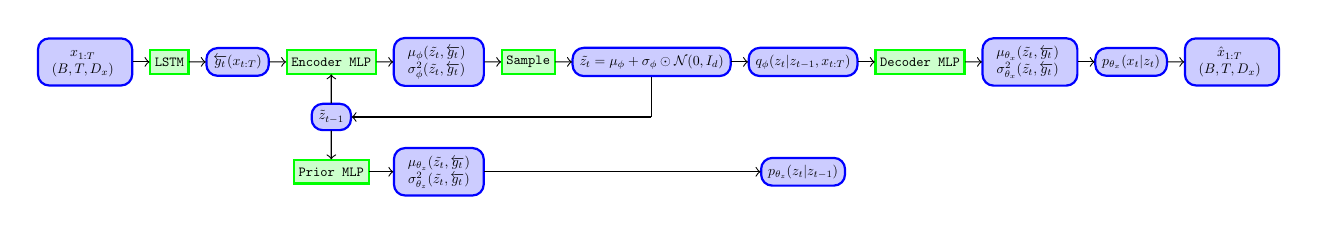
\begin{tikzpicture}[
    scale=0.70,
    every node/.style={scale=0.50},
    torch/.style={
        rectangle, 
        minimum size=6mm, 
        thick, 
        draw=green!100, 
        fill=green!20, 
        font=\ttfamily
        },
    math/.style={
        rectangle, 
        % minimum height=1cm,
        % minimum width=2cm,
        rounded corners, 
        thick, 
        draw=blue!100,
        fill=blue!20,
        align=center,
        anchor=center,
        inner sep=5pt
        },
    point/.style={
        circle,
        inner sep=0pt,
        minimum size=0pt,
        }
    ]
% \matrix[row sep = 1mm, column sep=5mm]{}
\matrix[row sep = 2mm, column sep=2mm]{
% first row
\node[math] (xt) {
    $\begin{array}{c}
            x_{1:T} \\
            (B,T,D_x)
    \end{array}$
}; &
\node[torch] (lstm) {LSTM}; & 
\node[math] (gt) {$\overleftarrow{g_t}(x_{t:T})$}; &
\node[torch] (enco) {Encoder MLP}; &
\node[math] (phi) {
    $\begin{array}{c}
            \mu_{\phi}(\tilde{z_t}, \overleftarrow{g_t}) \\
            \sigma_{\phi}^2(\tilde{z_t}, \overleftarrow{g_t})
    \end{array}$
}; &
\node[torch] (sample) {Sample}; &
\node[math] (z_tilde) {$\tilde{z_t}= \mu_{\phi} + \sigma_{\phi} \odot \mathcal{N}(0, I_d)$}; & 
\node[math] (q_phi) {$q_{\phi}(z_t \vert z_{t-1}, x_{t:T})$}; &
\node[torch] (deco) {Decoder MLP}; &
\node[math] (theta_x) {
    $\begin{array}{c}
        \mu_{\theta_x}(\tilde{z_t}, \overleftarrow{g_t}) \\
        \sigma_{\theta_x}^2(\tilde{z_t}, \overleftarrow{g_t})
    \end{array}$
}; &
\node[math] (p_theta_x) {$p_{\theta_x}(x_t \vert z_t)$}; &
\node[math] (x_hat) {
    $\begin{array}{c}
            \hat{x}_{1:T} \\
            (B,T,D_x)
    \end{array}$
}; \\
%second row
& & & \node[math] (z_t_1) (z_t_1) {$\tilde{z}_{t-1}$}; & & & \node[point] (coin) {}; & & &; \\
%third row
& & & \node[torch] (prior) {Prior MLP}; &
\node[math] (theta_z) {
    $\begin{array}{c}
            \mu_{\theta_z}(\tilde{z_t}, \overleftarrow{g_t}) \\
            \sigma_{\theta_z}^2(\tilde{z_t}, \overleftarrow{g_t})
    \end{array}$}; & & &
\node[math] (p_theta_z) {$p_{\theta_z}(z_t \vert z_{t-1})$}; &
& &; \\
};
\path   (xt) edge [->, thin] (lstm)
        (lstm) edge [->, thin] (gt)
        (gt) edge [->, thin] (enco)
        (enco) edge [->, thin] (phi)
        (phi) edge [->, thin] (sample)
        (sample) edge [->, thin] (z_tilde)
        (z_tilde) edge [->, thin] (q_phi)
        (q_phi) edge[->, thin] (deco)
        (deco) edge [->, thin] (theta_x)
        (theta_x) edge [->, thin] (p_theta_x)
        (p_theta_x) edge [->, thin] (x_hat)
        (z_t_1) edge [->, thin] (enco)
        (prior) edge [<-, thin] (z_t_1)
        (theta_z) edge [<-, thin] (prior)
        (theta_z) edge[->, thin] (p_theta_z)
        (z_tilde) edge [-, thin] (coin)
        (coin) edge [->, thin] (z_t_1);
\end{tikzpicture}
% --- Loss DKF
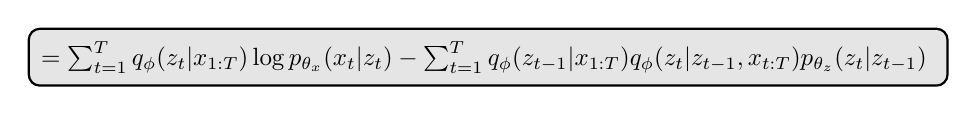
\begin{tikzpicture}[
    scale=0.90,
    every node/.style={scale=0.90},
    math/.style={
        rectangle, 
        % minimum height=1cm,
        % minimum width=2cm,
        rounded corners, 
        thick, 
        draw=black!100,
        fill=gray!20,
        align=center,
        anchor=center,
        inner sep=5pt
        },
    ]
    \node[math] {
            $\VLB = \sum_{t=1}^T \E{q_\phi(z_{t} \vert x_{1:T})} \log{p_{\theta_x}(x_t \vert z_t)} - \sum_{t=1}^T \E{q_\phi(z_{t-1} \vert x_{1:T})} \KL{q_{\phi}(z_t \vert z_{t-1}, x_{t:T})}{p_{\theta_z}(z_t \vert z_{t-1})}$
    };
\end{tikzpicture}
% % \end{centering}
% % \caption{Deep Kalman Filter Model Architecture}
\end{figure}
% % \end{landscape}
\end{frame}



% %
% %
% % ==========================================================
% %
% % === VARIATIONAL RNN ===
% %
% % ==========================================================
% %
% %

\begin{frame}{Second model : Variational RNN}
    \begin{itemize}
        \item The \gls{vrnn} is the most expressive \gls{dvae} : the general expressions \ref{gen_model_dvae}, \ref{inf_model_dvae} and \gls{vlb} \ref{vlb_dvae} can not be simplified.
        \item The \gls{gpm} of the \gls{vrnn} assumes full forward connections between latent variables, and between observed variables.
    \end{itemize}

\begin{figure}[h]
    \centering
    % \includegraphics[width=0.5\linewidth]{}
    \label{fig:graphical_model_vrnn}
\begin{tikzpicture}[
    HIDDEN/.style={circle, draw=black!0, thin, minimum size=10mm},
    UNOBS/.style={circle, draw=black!80, thin, minimum size=10mm},
    OBS/.style={circle, draw=black!80, fill=gray!50, thin, minimum size=10mm}
]
% nodes
\node[HIDDEN] (zs) {$...$}; % start z
\node[HIDDEN] (xs) [below= of zs] {$...$}; % start x
\node[UNOBS] (z_t_1) [right= of zs] {$z_{t-1}$} edge[<-, thin] (a);
\node[OBS] (x_t_1) [below= of z_t_1] {$x_{t-1}$}    edge[<-, thin] (z_t_1)
                                                    edge[<-, thin] (xs);
\node[UNOBS] (z_t)  [right= of z_t_1] {$z_{t}$} edge[<-, thin] (z_t_1)
                                                edge[<-, thin] (x_t_1);
\node[OBS] (x_t) [below= of z_t] {$x_{t}$}  edge[<-, thin] (z_t)
                                            edge[<-, thin] (x_t_1)
                                            edge[<-, thin] (z_t_1);
\node[UNOBS] (z_t_p1) [right= of z_t] {$z_{t+1}$}   edge[<-, thin] (z_t)
                                                    edge[<-, thin] (x_t);
\node[OBS] (x_t_p1) [below= of z_t_p1] {$x_{t+1}$}  edge[<-, thin] (z_t_p1)
                                                    edge[<-, thin] (x_t)
                                                    edge[<-, thin] (z_t);
\node[HIDDEN] (ze) [right= of z_t_p1] {$...$} edge[<-, thin] (z_t_p1); % end z
\node[HIDDEN] (xe) [right= of x_t_p1] {$...$} edge[<-, thin] (x_t_p1); % end x

\path[->]   (z_t_1) edge [bend left=+45] node[mid left] {} (z_t_p1)
            (x_t_1) edge [bend left=-45] node[mid left] {} (x_t_p1);
\end{tikzpicture}
\caption{Probabilistic model of a Variational RNN}
\end{figure}
\end{frame}

\begin{frame}{VRNN - Summary}
\begin{tcolorbox}[height=0.85\textheight, colback=blue!5!white,colframe=black!75!black,title=Variational RNN]
\fontsize{7pt}{8pt}\selectfont{
\begin{itemize}
    \item \textbf{generative model}
    \begin{align}
        \label{gen_model_vrnn}
        p_{\theta_x}(x_t \vert x_{1:t-1}, z_{1:t}) &= \NNdiag{x_t}{\mu_{\theta_x}(x_{1:t-1}, z_{1:t})}{\sigma_{\theta_x}^2(x_{1:t-1}, z_{1:t})} \\
        p_{\theta_z}(z_t \vert z_{1:t-1}, x_{1:t-1}) &= \NNdiag{z_t}{\mu_{\theta_z}(z_{1:t-1}, x_{1:t-1})}{\sigma_{\theta_z}^2(z_{1:t-1}, x_{1:t-1})}
    \end{align}
    \item \textbf{inference model}
    \begin{align}
        \label{inf_model_vrnn}
        q_{\phi}(z_{t} \vert z_{1:t-1}, x_{1:T}) &= \NNdiag{z_t}{\mu_{\phi}(z_{1:t-1}, x_{1:T})}{\sigma_{\phi}^2(z_{1:t-1}, x_{1:T})}
    \end{align}
    \item \textbf{\gls{vlb} for training}
    \begin{align}
        \label{vlb_vrnn}
        \begin{split}
        \VLB &= \sum_{t=1}^T  \E{q_{\phi}(z_{1:t} \vert x_{1:T})} \log{p_{\theta_x}(x_t \vert x_{1:t-1}, z_{1:t})} \\ &- \sum_{t=1}^T \E{q_{\phi}(z_{1:t-1} \vert x_{1:T})} \KL{q_{\phi}(z_t \vert z_{1:t-1}, x_{1:T})}{p_{\theta_z}(z_t \vert z_{1:t-1}, x_{1:t-1})}  \end{split}
    \end{align}
\end{itemize}
}
\end{tcolorbox}
\end{frame}

\begin{frame}[fragile]{VRNN - Torch}
    We have chosen a different implementation from \cite{girin_dynamical_2022} and used three different \gls{lstm} networks to encode $z_{1:t}$, $x_{1:t-1}$ and $x_{t:T}$ respectively.

    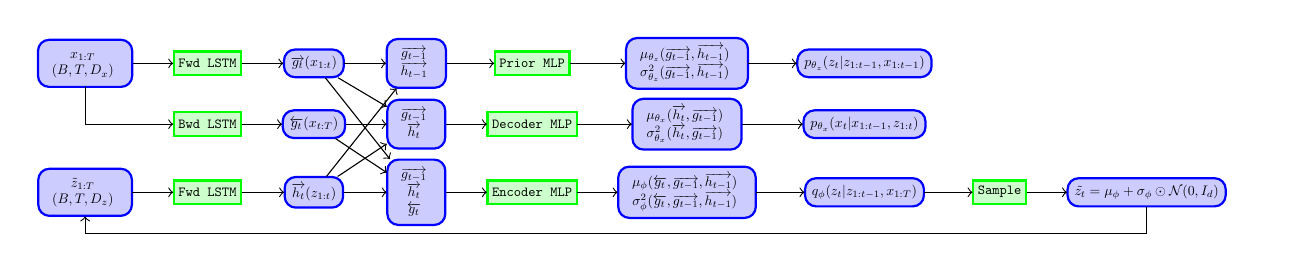
\begin{tikzpicture}[
    % format
    scale=0.50,
    every node/.style={scale=0.50},
    torch/.style={
        rectangle, 
        minimum size=6mm, 
        thick, 
        draw=green!100, 
        fill=green!20, 
        font=\ttfamily
        },
    math/.style={
        rectangle, 
        rounded corners, 
        thick, 
        draw=blue!100,
        fill=blue!20,
        align=center,
        anchor=center,
        inner sep=5pt
        },
    point/.style={
        circle,
        inner sep=0pt,
        minimum size=0pt,
        }
    ]
\matrix[row sep = 1mm, column sep=5mm] {
% row 1
\node[math] (xt) {
    $\begin{array}{c}
            x_{1:T} \\
            (B,T,D_x)
    \end{array}$
}; &
\node[torch] (fwd_lstm) {Fwd LSTM}; & 
\node[math] (gt) {$\overrightarrow{g_t}(x_{1:t})$}; &
\node[math] (g_t_1_et_h_t_1) {
    $\begin{array}{c}
        \overrightarrow{g_{t-1}} \\
        \overrightarrow{h_{t-1}}
    \end{array}$
}; &
\node[torch] (prior) {Prior MLP}; &
\node[math] (theta_z) {
    $\begin{array}{c}
            \mu_{\theta_z}(\overrightarrow{g_{t-1}}, \overrightarrow{h_{t-1}}) \\
            \sigma_{\theta_z}^2(\overrightarrow{g_{t-1}}, \overrightarrow{h_{t-1}})
    \end{array}$
}; &
\node[math] (p_theta_z) {$p_{\theta_z}(z_t \vert z_{1:t-1}, x_{1:t-1})$}; & \\
% row 2
\node[point] (coin3) {}; &
\node[torch] (bwd_lstm) {Bwd LSTM}; & 
\node[math] (gt2) {$\overleftarrow{g_t}(x_{t:T})$}; &
\node[math] (g_t_1_et_h_t) {
    $\begin{array}{c}
        \overrightarrow{g_{t-1}} \\
        \overrightarrow{h_{t}}
    \end{array}$
}; &
\node[torch] (decoder) {Decoder MLP}; &
\node[math] (theta_x) {
    $\begin{array}{c}
            \mu_{\theta_x}(\overrightarrow{h_t}, \overrightarrow{g_{t-1}}) \\
            \sigma_{\theta_x}^2(\overrightarrow{h_t}, \overrightarrow{g_{t-1}})
    \end{array}$
}; & 
\node[math] (p_theta_x) {$p_{\theta_x}(x_t \vert x_{1:t-1}, z_{1:t} )$}; & \\
% row 3
\node[math] (z_tilde) {
    $\begin{array}{c}
            \tilde{z}_{1:T} \\
            (B,T,D_z)
    \end{array}$
}; & 
\node[torch] (fwd_lstm2) {Fwd LSTM}; & 
\node[math] (ht) {$\overrightarrow{h_t}(z_{1:t})$}; &
\node[math] (g_t_1_et_h_t_1_et_g_t) {
    $\begin{array}{c}
        \overrightarrow{g_{t-1}} \\
        \overrightarrow{h_{t}} \\
        \overleftarrow{g_t}
    \end{array}$
}; &
\node[torch] (encoder) {Encoder MLP}; &
\node[math] (phi) {
    $\begin{array}{c}
            \mu_{\phi}(\overleftarrow{g_{t}}, \overrightarrow{g_{t-1}}, \overrightarrow{h_{t-1}}) \\
            \sigma_{\phi}^2(\overleftarrow{g_{t}}, \overrightarrow{g_{t-1}}, \overrightarrow{h_{t-1}})
    \end{array}$
}; & 
\node[math] (q_phi) {$q_{\phi}(z_t \vert z_{1:t-1}, x_{1:T} )$}; &
\node[torch] (sample) {Sample}; &
\node[math] (z_tilde_formula) {$\tilde{z_t} = \mu_{\phi} + \sigma_{\phi} \odot \mathcal{N}(0, I_d)$}; & \\
% row 4
\node[point] (coin1) {};
& & & & & & & &;
\node[point] (coin2) {}; & \\
};
\path   (xt) edge [->, thin] (fwd_lstm)
        (xt) edge[-, thin] (coin3)
        (fwd_lstm) edge [->, thin] (gt)
        (gt) edge[->, thin] (g_t_1_et_h_t_1)
        (gt) edge[->, thin] (g_t_1_et_h_t)
        (gt) edge[->, thin] (g_t_1_et_h_t_1_et_g_t)
        (g_t_1_et_h_t_1) edge[->, thin] (prior)
        (prior) edge[->, thin] (theta_z)
        (theta_z) edge[->, thin] (p_theta_z)
        (coin3) edge[->, thin] (bwd_lstm)
        (bwd_lstm) edge[->, thin] (gt2)
        (gt2) edge[->, thin] (g_t_1_et_h_t)
        (gt2) edge[->, thin] (g_t_1_et_h_t_1_et_g_t)
        (g_t_1_et_h_t) edge[->, thin] (decoder)
        (decoder) edge[->, thin] (theta_x)
        (theta_x) edge[->, thin] (p_theta_x)
        (z_tilde) edge[->, thin] (fwd_lstm2)
        (fwd_lstm2) edge[->, thin] (ht)
        (ht) edge[->, thin] (g_t_1_et_h_t_1_et_g_t)
        (ht) edge[->, thin] (g_t_1_et_h_t)
        (ht) edge[->, thin] (g_t_1_et_h_t_1)
        (g_t_1_et_h_t_1_et_g_t) edge[->, thin] (encoder)
        (encoder) edge[->, thin] (phi)
        (phi) edge[->, thin] (q_phi)
        (q_phi) edge[->, thin] (sample)
        (sample) edge[->, thin] (z_tilde_formula)
        (z_tilde_formula) edge[-, thin] (coin2)
        (coin2) edge[-, thin] (coin1)
        (coin1) edge[->, thin] (z_tilde);
\end{tikzpicture}


% LOSS

% --- Loss VRNN
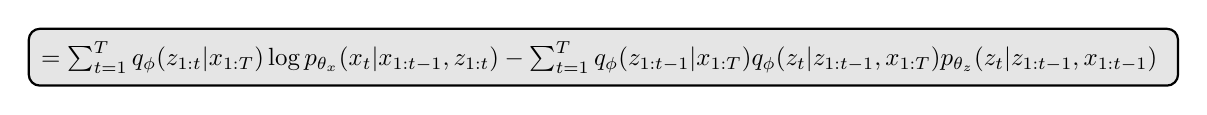
\begin{tikzpicture}[
    scale=0.90,
    every node/.style={scale=0.90},
    math/.style={
        rectangle, 
        % minimum height=1cm,
        % minimum width=2cm,
        rounded corners, 
        thick, 
        draw=black!100,
        fill=gray!20,
        align=center,
        anchor=center,
        inner sep=5pt
        },
    ]
    \node[math] {
        $\VLB = \sum_{t=1}^T  \E{q_{\phi}(z_{1:t} \vert x_{1:T})} \log{p_{\theta_x}(x_t \vert x_{1:t-1}, z_{1:t})} - \sum_{t=1}^T \E{q_{\phi}(z_{1:t-1} \vert x_{1:T})} \KL{q_{\phi}(z_t \vert z_{1:t-1}, x_{1:T})}{p_{\theta_z}(z_t \vert z_{1:t-1}, x_{1:t-1})}$
    };
\end{tikzpicture}

\end{frame}


% %
% %
% % ==========================================================
% %
% % === GAUSSIAN PROCESS VARIATIONAL AUTOENCODER ===
% %
% % ==========================================================
% %
% %

\begin{frame}{Third model : Gaussian Process - Variational Auto Encoder}
    \begin{figure}[H]
        \centering
        % \includegraphics[width=0.5\linewidth]{}
        \label{fig:graphical_model_gpvae}
    \begin{tikzpicture}[
        % scale=0.90,
        % every node/.style={scale=0.90},
        HIDDEN/.style={circle, draw=black!0, thin, minimum size=10mm},
        UNOBS/.style={circle, draw=black!80, thin, minimum size=10mm},
        OBS/.style={circle, draw=black!80, fill=gray!50, thin, minimum size=10mm}
    ]
    % nodes
        \node[HIDDEN] (a) {$...$};
        \node[UNOBS] (z_t_i_1) [right= of a] {$z_{t_{i-1}}$} edge[-, ultra thick] (a);
        \node[UNOBS] (z_t_i)  [right= of z_t_i_1] {$z_{t_i}$} edge[-, ultra thick] (z_t_i_1);
        \node[UNOBS] (z_t_i_p1) [right= of z_t_i] {$z_{t_{i+1}}$} edge[-, ultra thick] (z_t_i);
        \node[HIDDEN] (e) [right= of z_t_i_p1] {$...$} edge[-, ultra thick] (z_t_i_p1);
        \node[OBS] (x_t_i_1) [below= of z_t_i_1] {$x_{t_{i-1}}$} edge[<-, thin] (z_t_i_1);
        \node[OBS] (x_t_i) [below= of z_t] {$x_{t_i}$} edge[<-, thin] (z_t_i);
        \node[OBS] (x_t_i_p1) [below= of z_t_p1] {$x_{t_{i+1}}$} edge[<-, thin] (z_t_i_p1);
        \end{tikzpicture}
        \caption{Probabilistic model of a GP-VAE}
    \end{figure}

    \begin{itemize}
        \item \textbf{thick black lines} indicate a Gaussian Process prior over latent variables. 
        \item The joint distribution writes:
            \begin{align}
            \label{joint_gpvae}
                p(x_{t_1:t_T}, z_{t_1:t_T}) %&= p(z_{t_1:t_T}) p(x_{t_1:t_T} \vert z_{t_1:t_T}) \\
                %= p(z_{t_1:t_T}) \prod_{i=1}^T p(x_{t_i} \vert x_{t_1:t_{i-1}}, z_{t_1:t_T}) \\
                &= p(z_{t_1:t_T}) \prod_{i=1}^T p(x_{t_i} \vert z_{t_{i}})
            \end{align}
    \end{itemize}

\end{frame}


\begin{frame}{GP-VAE generative model}
    \begin{itemize}
        \item \textbf{Gaussian Process prior} : \textbf{the prior over the latent variables $z_{t_i} \in \R^L$ is a set of scalar Gaussian Process over each of the dimension $l \in \{1,...,L\}$ of the latent variables.} Formally:
            \begin{align}
                p_{\theta_z}(z_{t_1:t_T}^l) &= \mathcal{GP}(m_{\theta_z, l}(t_1:t_T), k_{\theta_z, l}(t_1:t_T, t_1:t_T)) \hspace{1cm} l=1,..,L
            \end{align}
            \begin{itemize}
                \item $m_{\theta_z, l}$ are the $L$ mean functions of the \gls{gp} priors (usually chosen constant null)
                \item $k_{\theta_z, l}$ are the kernel functions of the \gls{gp} priors. Can be chosen differently to account for prior knowledge of the data sequence.
                \item Each $\mathcal{GP}^l$ encode a temporal dependency over $z^{(l)}$
                \item Correlation accross dimensions of data is encoded within likelihood $p_{\theta_x}$
            \end{itemize}
        \item \textbf{Approximate posterior -encoder : $q_\phi$ is a set of $L$ Gaussian distributions of dimension $T$, each one accounting for a component of $z_{t_i}$.} Formally :
            \begin{align}
                q_\phi(z_{t_1:t_T}^l \vert x_{t_1:t_T}^l) &= \mathcal{N}(m_{\phi}^l(x_{t_1:t_T}), \Sigma_{\phi}^l(x_{t_1:t_T})) \hspace{1cm} l=1,..,L \\
                &= \mathcal{N}(m_{\phi}^l(x_{t_1:t_T}), \Lambda_{\phi}^l(x_{t_1:t_T})^{-1}) \\
                &= \mathcal{N}(m_{\phi}^l(x_{t_1:t_T}), L_{\phi}^l(x_{t_1:t_T})L_{\phi}^l(x_{t_1:t_T})^T)
            \end{align}
            Code covariance with covariance matrix $\Sigma_\phi^l$, precision matrix $\Lambda_\phi^l$, or with a Cholesky decomposition $L_{\phi}^lL_{\phi}^l$.
    \end{itemize}
\end{frame}

\begin{frame}{GP-VAE generative model}
    From \cite{li_disentangled_2018}
        \begin{figure}[H]
        \centering
        % \includegraphics[width=0.5\linewidth]{}
        \label{fig:schema_model_gpvae}
        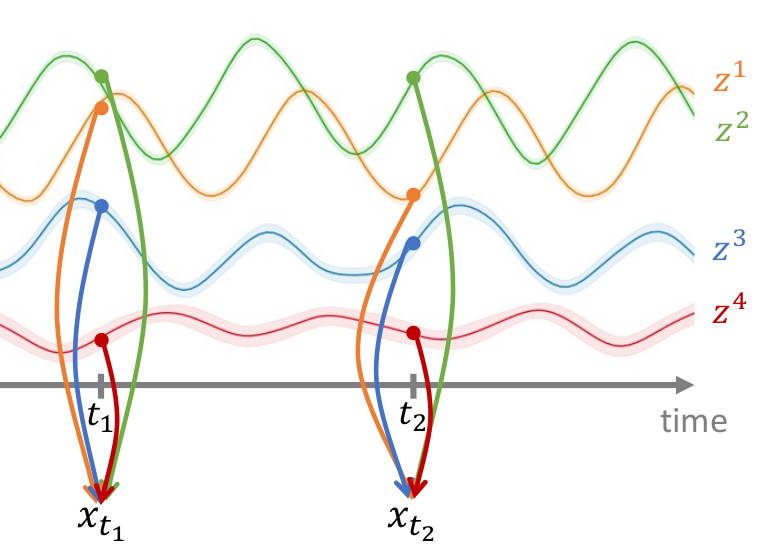
\includegraphics[width=0.5\textwidth]{/home/benjamin/Folders_Python/MVA/MVA_Stage/images/GP-VAE_schema.png}
        \caption{GP-VAE Schematics}
    \end{figure}
\end{frame}


\begin{frame}{GP-VAE likelihood and ELBO}
    \begin{align}
    \VLB = \sum_{i=1}^T \E{q_{\phi}(z_{t_i} \vert x_{t_1:t_T})} \log{p_{\theta_x}(x_{t_i} \vert z_{t_i})} - \KL{q_{\phi}(z_{t_1:t_T} \vert x_{t_1:t_T})}{p_{\theta_z}(z_{t_1:t_T})}
\end{align}
We note that:
\begin{itemize}
    \item the $\mathbb{KL}$-divergence is the sum of the $L$ $\mathbb{KL}$-divergences $\KL{q_{\phi}^l}{p_{\theta_z}^l}$ (close form solution)
    \item the negative log likelihood loss term requires sampling from $q_{\phi}(z_{t_i} \vert x_{t_1:t_T})$ using the reparameterization trick as usual.
    \item the \gls{gp} priors $p_{\theta_z}(z_{t_1:t_T})$ depend only on the time stamps $t_1,...t_T$. ($O(N^3)$ cost)
        \begin{itemize}
            \item If the kernel parameters are fixed -such as in \cite{fortuin_gp-vae:_2020}- then the priors can be computed before the training loop. 
            \item If the kernel parameters are learnt with the weights of the neural nets (such as in \cite{zhu_markovian_2023}), then the computation must occur at each training iteration.
        \end{itemize}
\end{itemize}
\end{frame}




\begin{frame}{GP-VAE Summary}
    \begin{tcolorbox}[height=0.85\textheight,colback=blue!5!white,colframe=black!75!black,title=Gaussian Process VAEs]
    % \begin{itemize}
    %     \item \textbf{generative model}
    \fontsize{7pt}{8pt}\selectfont{
        \begin{align}
            \label{gen_model_gpvae}
            p(x_{t_1:t_T}, z_{t_1:t_T}) &= p(z_{t_1:t_T}) \prod_{i=1}^T p(x_{t_i} \vert z_{t_{i}}) \\
            p_{\theta_z}(z_{t_1:t_T}^l) &= \mathcal{GP}(m_{\theta_z, l}(t_1:t_T), k_{\theta_z, l}(t_1:t_T)) \hspace{1cm} l=1,..,L
        \end{align}
        % \item \textbf{inference model}
        \begin{align}
            \label{inf_model_gpvae}
            q_\phi(z_{t_1:t_T}^l \vert x_{t_1:t_T}^l) &= \mathcal{N}(m_{\phi}^l(x_{t_1:t_T}), \Sigma_{\phi}^l(x_{t_1:t_T})) \hspace{1cm} l=1,..,L \\
            &= \mathcal{N}(m_{\phi}^l(x_{t_1:t_T}), \Lambda_{\phi}^l(x_{t_1:t_T})^{-1}) \\
            &= \mathcal{N}(m_{\phi}^l(x_{t_1:t_T}), L_{\phi}^l(x_{t_1:t_T})L_{\phi}^l(x_{t_1:t_T})^T)
        \end{align}
        % \item \textbf{\gls{vlb} for training}
        \begin{align}
            \label{vlb_gpvae}
            \VLB = \sum_{i=1}^T \E{q_{\phi}(z_{t_i} \vert x_{t_1:t_T})} \log{p_{\theta_x}(x_{t_i} \vert z_{t_i})} - \KL{q_{\phi}(z_{t_1:t_T} \vert x_{t_1:t_T})}{p_{\theta_z}(z_{t_1:t_T})} 
        \end{align}
    % \end{itemize}
    }
    \end{tcolorbox}
\end{frame}

\begin{frame}[fragile]{GP-VAE - Torch}
    \begin{tikzpicture}[
    % format
    scale=0.30,
    every node/.style={scale=0.30},
    torch/.style={
        rectangle, 
        minimum size=6mm, 
        thick, 
        draw=green!100, 
        fill=green!20, 
        font=\ttfamily
        },
    math/.style={
        rectangle, 
        rounded corners, 
        thick, 
        draw=blue!100,
        fill=blue!20,
        align=center,
        anchor=center,
        inner sep=5pt
        },
    point/.style={
        circle,
        inner sep=0pt,
        minimum size=0pt,
        }
    ]
    % place nodes
    \matrix[row sep = 1mm, column sep=5mm] {
    % % row 1
        \node[math] (xt) {
        $\begin{array}{c}
                x_{t_1:t_T} \\
                (B,T,D_x)
        \end{array}$
        }; &
        \node[torch] (encoder) {
        $\begin{array}{c}
            \text{\ttfamily{Encoder MLP}} \\
            + \, \text{\ttfamily{torch.permute}}
        \end{array}$
        }; &
        \node[math] (zt_perm) {
        $\begin{array}{c}
                z_{t_1:t_T} \\
                (B,D_z,T)
        \end{array}$
        }; & 
        \node[math] (phi) {
            $\begin{array}{c}
                    \mu_{\phi}^l(x_{t_1:t_T}) \,\,\, (B,D_z,T)\\
                    \Sigma_{\phi}^l(x_{t_1:t_T}) \,\,\, (B,D_z,T,T) \\
                    l=1,...,D_z
            \end{array}$
        }; & 
        \node[math] (q_phi) {
        $\begin{array}{c}
        q_{\phi}^l(z_{t_1:t_T} \vert x_{t_1:t_T} ) \\
        (B,D_z) \times \mathcal{N}(T, T\times T)
        \end{array}$
        }; &
        \node[torch] (sample) {
        $\begin{array}{c}
        \text{\ttfamily{Sample}} \\
        + \, \text{\ttfamily{torch.permute}}
        \end{array}$
        }; &
        \node[math] (zt_tilde_perm) {
        $\begin{array}{c}
                \tilde{z}_{t_1:t_T} \\
                (B,T,D_z)
        \end{array}$
        }; & 
        \node[torch] (decoder) {Decoder MLP}; &
        \node[math] (theta_x) {
            $\begin{array}{c}
                    \mu_{\theta_x}^t(z_{t_1:t_T}) \,\,\, (B,T,D_x)\\
                    \Sigma_{\theta_x}^t(z_{t_1:t_T}) \,\,\, (B,T,D_x,D_x) \\
                    t=1,...,T
            \end{array}$
        }; & 
        \node[math] (p_theta_x) {
        $\begin{array}{c}
        p_{\theta_x}(x_{t_1:t_T} \vert \tilde{z}_{t_1:t_T} ) \\ 
        (B,T) \times \mathcal{N}(D_x, D_x\times D_x) \\
        \end{array}$
        }; & \\
    % row 2
    \node[math] (times) {
        $\begin{array}{c}
                {t_1:t_T} \\
                (B,T,1)
        \end{array}$
        }; & &  
    \node[torch] (prior) {GP Prior}; &
    \node[math] (theta_z) {
            $\begin{array}{c}
                    m_{\theta_z, l}({t_1:t_T}) \,\,\, (B,D_z,T)\\
                    k_{\theta_z, l}({t_1:t_T,t_1:t_T}) \,\,\, (B,D_z,T,T) \\
                    l=1,...,D_z
            \end{array}$
        }; &  
    \node[math] (p_theta_z) {
        $\begin{array}{c}
        p_{\theta_z}({t_1:t_T}) \\ 
        (B,D_z) \times \mathcal{N}(T, T\times T) \\
        \end{array}$
        }; & \\
    };
    % draw edges
    \path   (xt) edge [->, thin] (encoder)
            (encoder) edge [->, thin] (zt_perm)
            (zt_perm) edge [->, thin] (phi)
            (phi) edge [->, thin] (q_phi)
            (q_phi) edge [->, thin] (sample)
            (sample) edge [->, thin] (zt_tilde_perm)
            (zt_tilde_perm) edge [->, thin] (decoder)
            (decoder) edge [->, thin] (theta_x)
            (theta_x) edge [->, thin] (p_theta_x)
            (times) edge[->, thin] (prior)
            (prior) edge[->, thin] (theta_z)
            (theta_z) edge[->, thin] (p_theta_z);
\end{tikzpicture}


% --- Loss GPVAE
\begin{figure}[h]
    \centering
    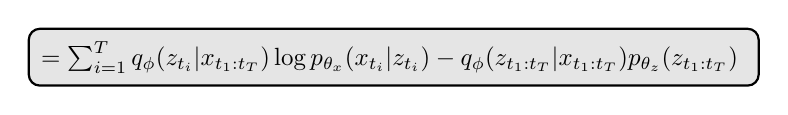
\begin{tikzpicture}[
    scale=0.90,
    every node/.style={scale=0.90},
    math/.style={
        rectangle, 
        % minimum height=1cm,
        % minimum width=2cm,
        rounded corners, 
        thick, 
        draw=black!100,
        fill=gray!20,
        align=center,
        anchor=center,
        inner sep=5pt
        },
    ]
    \node[math] {
        $\VLB = \sum_{i=1}^T \E{q_{\phi}(z_{t_i} \vert x_{t_1:t_T})} \log{p_{\theta_x}(x_{t_i} \vert z_{t_i})} - \KL{q_{\phi}(z_{t_1:t_T} \vert x_{t_1:t_T})}{p_{\theta_z}(z_{t_1:t_T})}$
    };
\end{tikzpicture}
\end{figure}

\end{frame}